\documentclass[a4paper, openany]{memoir}

\usepackage[utf8]{inputenc}
\usepackage[T1]{fontenc} 
\usepackage[english]{babel}
\usepackage{amsmath}
\usepackage{amssymb}

\usepackage{booktabs}
\usepackage{fancyhdr}
\usepackage{float}
\usepackage{indentfirst}
\usepackage{graphicx}
\usepackage[linewidth=1pt]{mdframed}
\usepackage{multicol}
\usepackage{fancyvrb}

\pagestyle{fancy}
\fancyhf{}
\fancyhead[LE]{\leftmark}
\fancyhead[RO]{\rightmark}
\fancyhead[RE, LO]{PSD}
\fancyfoot[LE, RO]{\thepage}
\fancyfoot[RE, LO]{Pete Gautam}

\renewcommand{\headrulewidth}{1.5pt}

\chapterstyle{thatcher}
\setcounter{chapter}{4}

\begin{document}

\chapter{Customer Management}
Customers come in all shapes and sizes. They have different experiences and expectations. In particular,
\begin{itemize}
    \item they may not know what is realistic;
    \item they may not know how to explain what they really want (or the team might misunderstand them);
    \item they may change their mind frequently; and
    \item they may not be reliable.
\end{itemize}
According to Dawson (2000), the customer isn't trying to be difficult- they're being real. 

The team is responsible for managing the customer's expectations and a realistic workload. The team should also:
\begin{itemize}
    \item be flexible, but realistic, about requirements change; and
    \item be prepared to say something that isn't possible.
\end{itemize}
It is up to the team to ensure that the customer delivers on their commitments.

The team should understand the customer's priorities. Within a fixed time frame, what are they wanting:
\begin{itemize}
    \item Is it a proof of concept prototype? That is, a feature-rich software that may not very reliable.
    \item Is it a sustainable basis for future development? That is, the software is to be used by a lot of customers (and will have a smaller feature set)- it is suited for maintenance and future development.
\end{itemize}
In general, the customer can only expect to choose 2 from: a high quality, a quick and a complete software.

\section{Intellectual Property and Licensing}
Intellectual property (IP) is a complex issue in a collaborative projects- the key is for both parties to be reasonable. Both parties (customer and team) may contribute background IP (what they bring to the project). There is also foreground IP- what gets created during the process. If there is a transfer of IP from the team to the customer, then the team should be compensated. However, open source licenses are often the best solution. Many customers lack the capability to exploit the IP. Using open source means that the project is available for both parties to use in future. Both parties benefit by learning about the product/technology, even though neither side benefits from the IP.

The key thing to check to decide for the IP is:
\begin{itemize}
    \item is the project likely to have direct commercial value to either party?
    \item is the customer at a position to further exploit outputs at the end?
\end{itemize}

We will consider 3 examples and decide the IP:
\begin{itemize}
    \item \begin{figure}[H]
        \centering
        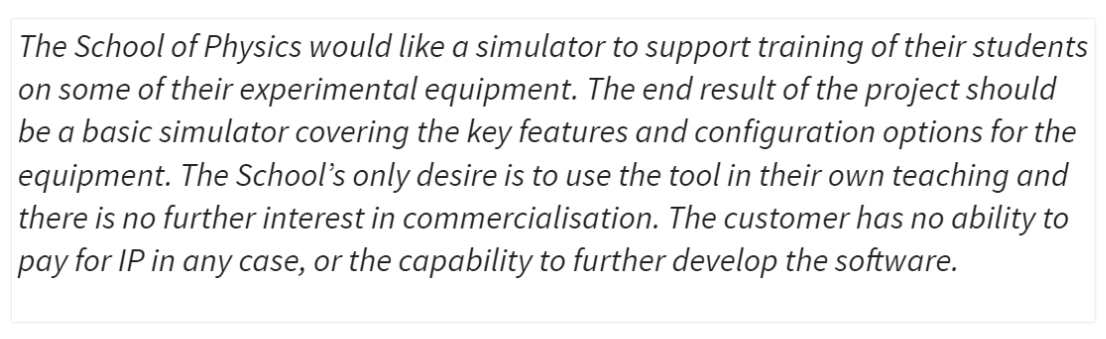
\includegraphics[scale=0.45]{src/IP Example 1.PNG}
    \end{figure}
    In this case, we probably have no commercial benefit- this should be open source.
    
    \item \begin{figure}[H]
        \centering
        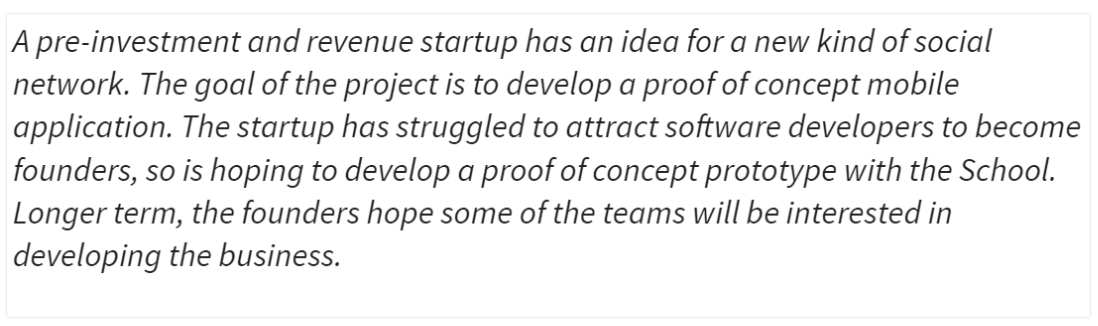
\includegraphics[scale=0.45]{src/IP Example 2.PNG}
    \end{figure}
    In this case, we should either use open source licensing or IP sharing. The customer benefits from what can be built, and the developers gain experience, and the project might be part of the startup.
    
    \item \begin{figure}[H]
        \centering
        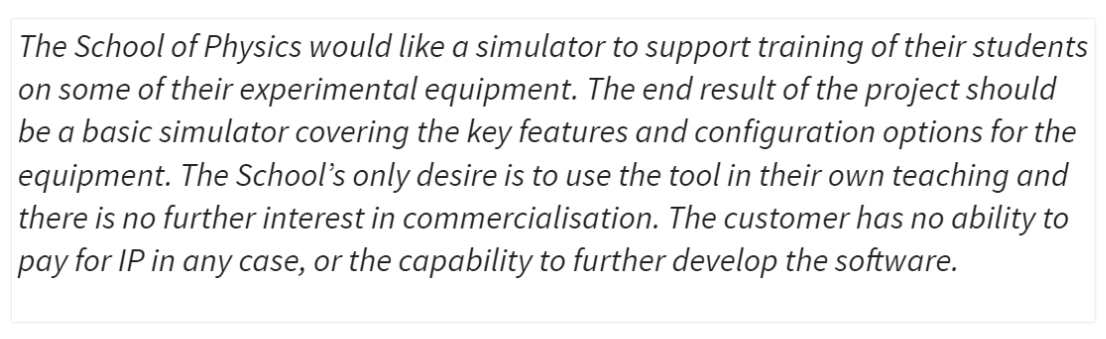
\includegraphics[scale=0.45]{src/IP Example 1.PNG}
    \end{figure}
    In this case, there should be an IP transfer.
\end{itemize}

\section{Review and Planning Meetings}
The review meeting is used to review progress since the last meeting. In particular, the team can discuss:
\begin{itemize}
    \item what they achieved and how that differs from what was agreed in the previous meeting;
    \item what additional work the team did in the last iteration;
    \item what the reasons for deviation were.
\end{itemize}
It is also a time to discuss the key new requirements:
\begin{itemize}
    \item the new features that emerge from the review;
    \item obstacles that have been uncovered (before making progress).
\end{itemize}
Then, the team can agree on a plan for the next iteration. The team should have a proposal ready, but negotiate with the customer to finalise it. The team can discuss new features and other enhancements. There might be significant defects to be fixed.

\section{Roles in a customer meeting}
The following are roles in a customer meeting:
\begin{itemize}
    \item the chair manages the agenda, keeps the meeting to time, and constrains discussions so that the meeting doesn't overrun;
    \item the product owner (who may combine with the chair) is the chief negotiator with the customer; 
    \item the lead demonstrator (who is different to the chair) demonstrates the product;
    \item the note taker takes notes during the meeting; and
    \item the checker ensures that nothing has been missed during the meeting.
\end{itemize}

\section{Agenda}
The agenda is a good way to summarise the agenda at the start. The agenda should be specific to the project, e.g. it should summarise what was done in the iteration, what was not done in the iteration, and what will be done in the next iteration. It is also a place to signpost any questions the customer will be asked to resolve during the meeting.

It is a good practice to estimate the time taken for each item and record it in the agenda- this is time boxing. The chair is responsible for ensuring that nothing goes over. It helps the team decide how best to use the time doing the meeting. Moreover, it helps the chair decide when to pause a discussion of the agenda item. 

Discussions that overrun should be paused. Extra time should be used at the end if available. Otherwise, the team should resolve the issue later (before the next meeting) with the customer.

\section{Managing discussion}
During the meeting, a careful balance needs to be be made between ensuring useful ideas and suggestions are discussed, and preventing a discussion from deviating too much from the agenda.

It is the chair's job to:
\begin{itemize}
    \item interrupt a speaker (including the customer) if the chair believes they have talked too much;
    \item ask the customer to elaborate more if the chair doesn't think the point has been clarified; and
    \item ask someone to contribute to simulate discussion.
\end{itemize}

\section{Effective Requirements Gathering}
It is a good idea to use visual aides (e.g. wireframes) to focus the customer's attention during different phases of the meeting. Moreover, customer meetings should be used to highlight complex decisions. It is a good idea to experiment structured technologies, e.g. value proposition canvas, user study workshop, design studies, etc. Also, it is good to have a live walkthrough of new features to illustrate progress. Moreover, the customer should be given the ability to interact with the product before/during the meeting.

It is also a good idea to ask focused questions. For example, instead of asking ``Do you like the user interface design?'', it is better to ask ``Which part of these 3 user interface mask-ups do you prefer?''- giving choices is better to elicit customer preferences. Moreover, instead of asking ``Which of the 10 features would you like?'', it is better to ask ``Which two features should be implemented first? Which two after that?''- this forces the customer to rank what they would like implemented. Also, instead of asking ``The system will have a mobile user interface, right?'', it is better to ask ``A mobile application will be the only user interface, right''- the questions should be clear.

\section{Documenting meeting}
Note taking should be the only job for at least one person. Moreover, it is a good idea to record the meeting, with the customer's permission.

\section{Setting a plan}
The team should have a project proposal ready for next sprint. This can incorporate what the team believes is important:
\begin{itemize}
    \item work delayed from previous sprints;
    \item existing backlog items; and
    \item new features identified during the previous sprint.
\end{itemize}
Also, the team should anticipate the priority of work items to be changed by the customer. The customer might want things to be prioritised differently. It is important to be realistic with the customer in terms of the time available. In particular,
\begin{itemize}
    \item the team should ensure the total amount of work planned is less than the available time;
    \item the team should have person-time estimates for each proposed work item.
\end{itemize}

It is important to negotiate the plan with the customer. The customer's expectations and priorities will vary from the team's preference at some point. Radical changes in direction (due to some opportunity) should be approached cautiously. The team shoul-dn't agree immediately to the customer's plan if the impact of the change isn't clear. The team should take time to evaluate the impact on their schedule. Also, they should be honest with the customer about the choice to be made. They should be prepared to negotiate a new schedule with the customer during the meeting. They should incorporate delays into new schedules.

\section{Managing meeting outcomes}
At the end of the meeting, the team should summarise their overall goal and work items to the customer. They should create backlog items for newly agreed work items. The team should create issues for follow-up takes, e.g. additional meetings and resource requests before they become blockers.

In summary, managing customers and expectations requires preparation and organisation. Customers aren't being deliberately difficult- they're just being human.

\end{document}